\lab{Algorithms}{Temporal Complexity and Sparse Matrices}{Complexity and Sparse Matrices}

\objective{It also introduces the concept of temporal complexity.
Finally, it explores SciPy's special methods for working with sparse matrices.}

\section*{Temporal Complexity}
One of the most important questions in scientific computing is:
How long will this operation take?
The concept of temporal complexity attempts to answer this question by determining
how much time a function needs to operate on a given size of input.
For example suppose calculating the inverse of a matrix of size $n$ (that is, an $n \times n$ matrix)
requires the following number of calculations.
\begin{equation*}
f(n) = \frac{3n^3}{2} + 75n^2 + 250n + 30
\end{equation*}
What is the most important part of this expression?
When our input gets very large the only relevant term in this equation is $n^3$.
For this reason we say that $f(n) \in O(n^3)$, or more commonly that $f(n)$ is $O(n^3)$
(spoken ``Big O of n cubed'' or ``order of n cubed").
This notation is borrowed from analysis. The notation captures the salient behavior of our temporal complexity,
or more precisely the growth rate we can expect of the execution time of our algorithm.
We also refer to this as \emph{asymptotic notation}.
We will discuss this concept later, but this is a simple introduction to the notion of complexity and Big O.
\begin{figure}[h]
\centering
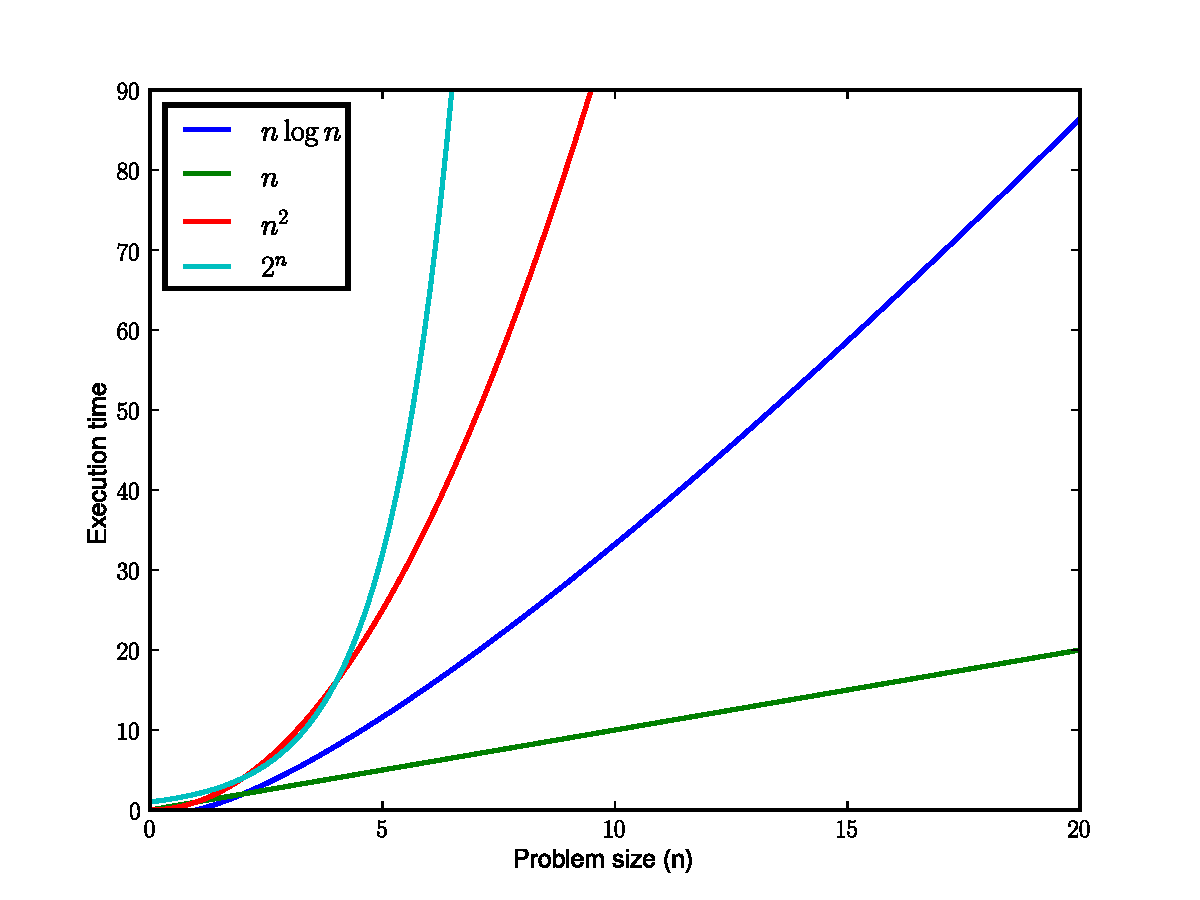
\includegraphics[width=\textwidth]{complexitycurves.pdf}
\caption{Some common asymptotic curves.}
\end{figure}

\begin{definition}[Temporal Complexity]
Let $n$ represent the problem size.  Let $f(n)$ and $g(n)$ be functions mapping natural numbers to positive real numbers. We say that $f \in O(g(n))$ if there exists a real
number $c > 0$ and a natural number $n_0$ such that for all natural numbers $n > n_0$,
$f(n) \leq cg(n)$.
When this is satisfied, we say that $g(n)$ is an asymptotic upper bound for $f(n)$.
The notation $f = O(g(n))$ is also common.
\end{definition}

\begin{problem}
Verify the following relationships
\begin{itemize}
\item $O(\log{n}) \subset O(n) \subset O(n\log{n})$
\item $O(n^k) \subset O(n^{k+1})$
\item $O(n^p) \subset O(2^n)$ for all $p \in \mathbb{N}$
\end{itemize}
\end{problem}

What does this have to do with computer programs?
Every algorithm executed on a computer corresponds to a function
that returns the number of steps taken (and therefore the time)
given an input of size $n$.  Certain problems can be solved with fewer steps,
while others require many more.  For example, given two matrices of size $n$,
it takes about $n^2$ steps to add the entries together and thus matrix addition is $O(n^2)$.
On the other hand, it takes about $n^3$ steps to calculate the inverse using Gaussian
row reduction, and thus this algorithm is $O(n^3)$. (There are in fact more efficient
algorithms for matrix inversion, and the question of the optimal asymptotic bound remains open.)

How do we determine the temporal complexity of a piece of code?
Calculating the exact temporal complexity of a formula is fairly difficult.
However, to asymptotically analyze a function is fairly straightforward.
\begin{lstlisting}
s = 0
for i in xrange(100):
    s = s + i
\end{lstlisting}
The code above is $O(n)$ because it takes approximately $n$ steps to complete its work.
For-loops are a good indicator of the complexity.  A double for-loop strongly suggests
$O(n^2)$ or worse.  The reason that array addition is $O(n^2)$ is because we have to add
$n^2$ elements for size $n \times n$ arrays.  Asymptotic analysis reveals that
if we have an array of size $n \times n$ and it takes $x$ seconds to execute an $O(n^2)$ algorithm,
then by increasing the size of the array to $2n \times 2n$, we should expect the same algorithm
to terminate in about $(2)^2 x = 4x$ seconds.  Sometimes, when you don't have code to look at,
you can approximate the asymptotic growth of a function by timing it on various sized inputs.

\begin{problem}
Determine the asymptotic growth of the following code that calculates all the partial sums
up to 1000.
\begin{lstlisting}
t = 0
for n in xrange(1000):
    t += sum(xrange(n))
\end{lstlisting}
%the asymptotic growth is $O(n^2)$
\end{problem}

We can also classify an algorithm by the amount of memory it needs to execute.  We will use the term \emph{spatial complexity} to measure the amount of memory an algorithm uses.  The definition of spatial complexity is the same as the definition for temporal complexity with the obvious difference that $n$ refers to space rather than time.
In practice, spatial and temporal complexity are not completely independent of each
other. The amount of memory required by an algorithm can affect its speed in several
ways. The most important consideration is that when the memory usage exceeds the amount
of available RAM, the machine must use the hard disk or some other slower storage
method, and read and write operations become substantially slower.

\section*{Sparse Matrices}
A sparse matrix is a matrix that has relatively few nonzero elements.
SciPy has several different ways of storing sparse matrices.
Each way has it pros and cons (the reader is encouraged to read the help for each way).

\begin{table}[h!]
\centering
\begin{tabular}{|l|l|}
\hline
Function & Description \\
\hline
\li{sparse.bsr()} & Compressed Block Sparse Row\\
\li{sparse.coo()} & Coordinate\\
\li{sparse.csc()} & Compressed Sparse Column\\
\li{sparse.csr()} & Compress Sparse Row\\
\li{sparse.dia()} & Sparse Diagonal\\
\li{sparse.dok()} & Dictionary of Keys\\
\li{sparse.lil()} & Linked List\\
\hline
\end{tabular}
\caption{Sparse matrix representations in SciPy}
\end{table}
Type the following into IPython.
\begin{lstlisting}
>>> from scipy import sparse
>>> A = np.diagflat([2,3,4])
>>> B = sparse.csc_matrix(A)
>>> C = B.todense()
\end{lstlisting}
Notice that the matrix $A$ has only three non-zero entries, and so we can consider it sparse.
In memory, an array stores a piece of data (be it an integer, float, or complex number)
in each entry, meaning that a $3 \times 3$ matrix requires a total 9 blocks of memory.
However, if we leverage the sparsity of $A$ we realize that we only need to store 3 numbers.
The \li{sparse} methods do exactly this: they store only the non-zero entries and their locations in the matrix.
No longer are storing an entire array.  SciPy has many methods for performing operations on sparse matrices.
To convert back to a dense matrix, we use the \li{todense()} method of the sparse matrix.
We can also convert between the different types sparse matrices.

We remark that if you want to make a sparse diagonal matrix, the
best way to do it isn't to use \li{diagflat()} followed by \li{sparse},
it's actually better to use the \li{sparse.spdiags()} method:
\begin{lstlisting}
>>> sparse.spdiags([2,3,4],0,3,3)
\end{lstlisting}
Often, when we are using sparse matrices, we are dealing with matrices
that are too large to be handled efficiently when represented in full form.

%insert problem here that lets them play around with large sparse matrices in diff forms

\section*{Banded Matrices}
A banded matrix is one whose only non-zero entries are diagonal
strips.  For example, the matrix
\begin{equation*}
A = \begin{pmatrix}
1 & 2 & 0 & 0 \\
3 & 4 & 5 & 0 \\
0 & 6 & 7 & 8 \\
0 & 0 & 9 & 10
\end{pmatrix}
\end{equation*}
is banded because there are three nonzero diagonals.  This
particular type of banded matrix is called a tri-diagonal matrix.

You can easily create banded matrices using the \li{diagflat()} method.
For example, the matrix $A$ above can be created by entering
\begin{lstlisting}
>>> np.diagflat([3, 6, 9], -1) + np.diagflat([1, 4, 7, 10], 0) + np.diagflat([2, 5, 8], 1)
\end{lstlisting}

Often a better way to create a tri-diagonal is it use the \li{sparse.spdiags()} method.
This is because many banded matrices are sparse.
For example, we create the same matrix using the command:
\begin{lstlisting}
>>> Z = np.array([[3, 1, 0], [6, 4, 2], [9, 7, 5], [0, 10, 8]]).T
>>> sparse.spdiags(Z, [-1, 0, 1], 4, 4)
\end{lstlisting}

For more information, check the documentation by typing \li{sparse.spdiags?}.
For example we create a tri-diagonal array with uniformly distributed random entries.
This example also demonstrates the efficiency of using sparse arrays.
\begin{lstlisting}
>>> B = np.rand(3,10000)
>>> A = sparse.spdiags(B, range(-1, 2), 10000, 10000)
>>> denseA = A.todense()  #only do this step if you have _lots_ of memory!
>>> A.data.nbytes
240000          #about 0.24MB of memory
>>> denseA.nbytes
800000000       #about 762.9MB of memory!
\end{lstlisting}
Although the complete matrix is too large to represent in memory,
we can still visualize it using the \li{plt.spy()} command from Matplotlib,
which essentially shows the location of non-zero entries in a matrix.
The output of \li{plt.spy(A)} in this case is shown in Figure \ref{fig:mpl_spy}.
\begin{figure}[h]
\centering
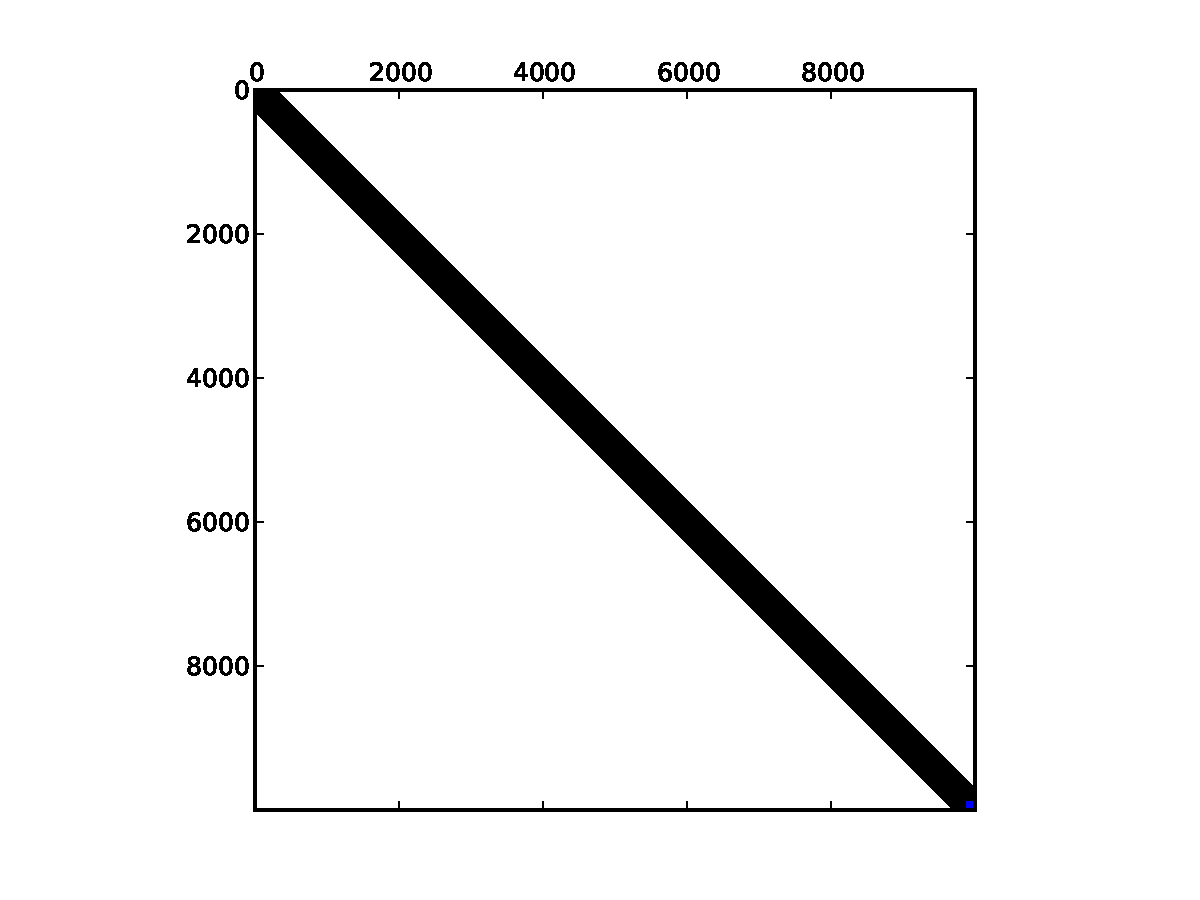
\includegraphics[width=\textwidth]{spy.pdf}
\caption{The output of the \li{spy()} command}
\label{fig:mpl_spy}
\end{figure}

\section*{Using Sparse Matrices}
Consider the linear system $A x = b$, where $A$ is a $100000\times 100000$ tri-diagonal matrix.
To store a full matrix of that size in your computer, it would normally require 10
billion double-precision floating-point numbers.  Since it takes 8
bytes to store a double, it would take roughly 80GB to store the
full matrix.  For most desktop computers, that fact alone makes the
system numerically prohibitive to solve.
The temporal complexity of the problem is even more problematic.
Methods for directly solving an arbitrary linear system are usually $O(n^3)$.
As a result, even if the computer could store an 80GB matrix in RAM, it
would still take several weeks to solve the system.  However, since
we don't have computers with that much available RAM, most of the
matrix would have to be stored on the hard drive, so the computation
would probably take between $6$ months to a year.

The point is that even the next generation of computers will
struggle with solving arbitrary linear systems of this size in a
reasonable period of time.  However, if we take advantage of the
sparse structure of the tri-diagonal matrix, we can solve the linear
system, even with a modest modern computer.  This is because all of
those zeros don't need to be stored and we don't need to do as many
operations to row reduce the tri-diagonal system.

Let's first compute the spatial complexity of the above system when
considered as a sparse matrix.  There are three diagonals that have
roughly $100000$ non-zero entries.  That's $300000$
double-precision floating point numbers, which is about 2.4 MB (Less
storage than your favorite song).  As a result, it will easily
fit into the computer's RAM.  Furthermore, the temporal complexity for solving
a tri-diagonal matrix is $O(n)$. Let's see how long it takes to
solve the system for random data:
\begin{lstlisting}
>>> import scipy as sp
>>> from scipy import sparse as spar
>>> from scipy.sparse import linalg as sparla
>>> D = sp.rand(3, 100000)
>>> b = sp.rand(1, 100000)
>>> A = spar.spdiags(D,[-1,0,1],100000,100000)
>>> def solSys():
>>>     return sparla.spsolve(A,b)
>>> %timeit solSys()
\end{lstlisting}

\begin{problem}
Write a function that returns a full $n\times n$
tri-diagonal array with $2$'s along the diagonal and $-1$'s along
the two sub-diagonals above and below the diagonal.
\label{prob:full_tridiag}
\end{problem}

\begin{problem}
Write another function that builds the same array as above, but as a sparse array.
You must build this as a sparse matrix from the beginning.
Hint: Use the \li{spar.spdiags()} method.
\label{prob:sparse_tridiag}
\end{problem}

\begin{problem}
Solve the linear system $Ax = b$ where $A$ is the $n\times n$
tri-diagonal array from Problem \ref{prob:full_tridiag} and Problem \ref{prob:sparse_tridiag} and $b$ is randomly
generated.  How high can you go for each method?  Make a table for
several different values of $n$ and the time it took to solve for
each run.  What conclusions can you draw?
\end{problem}

\begin{problem}
Using the sparse array above and the method \li{sparla.eigs},
calculate the smallest eigenvalue $\lambda$ of the array as the array's size goes to infinity. (You will need to set the \li{which = 'SM'} optional argument.) 
What value does $\lambda n^2$ approach?
Hint: It's the square of an important number.
This is related to operator theory: the second derivative operator has this eigenvalue in certain cases.
\end{problem}

\section*{Other Sparse Commands}
One important method of sparse matrix objects is the \li{nonzero()} method,
which is related to the number of nonzero entries in the matrix.
This number is important because it is an indicator of the amount of time and space
that is required to operate on the sparse matrix.
You should be aware that there is some overhead to using and storing the sparse matrix data structure.
Sparsely represented matrices are very beneficial when the number of
nonzero entries is relatively small compared to the total number of entries.
When the matrix has many nonzero entries, a sparse representation becomes disadvantageous.
To see this, create and execute a script with the following code:
\begin{lstlisting}
>>> A = np.random.rand(600,600)
>>> B = spar.csc_matrix(A)
>>> def square(A):
>>>     return sp.power(A, 2)
>>> %timeit square(A)
>>> %timeit square(B)
\end{lstlisting}
Run the script and note the two different runtimes.
Notice that it takes much longer to square the sparse matrix.
This is because the sparse matrix data structure is optimized for matrices that are actually sparse.
The array $A$ is entirely nonzero.
Thus, you incur the overhead of the sparse array representation without any
benefits since there are no entries you are not required to store or compute.
To summarize, only use a sparse matrix when your matrix is in fact sparse.
Using sparse matrices for mostly nonzero arrays will negatively impact performance and memory requirements.

Just as with dense arrays, we can pre-allocate sparse matrices.
Sometimes it is necessary to create sparse matrices that do not have a nice banded pattern.
We initialize a sparse matrix just like any other array.
The most efficient sparse matrix for pre-allocation is LIL.
Once you are done constructing you sparse matrix and wish to perform calculations,
you should convert to a more efficient sparse matrix (CSR or CSC).
\begin{lstlisting}
>>> Z = spar.lil_matrix((400,300))
<400x300 sparse matrix of type '<type 'numpy.float64'>'
        with 0 stored elements in Linked List format>
>>> Z[1,34] = 23
>>> Z[23,32] = 56
>>> Z[2,:] = 13.2
\end{lstlisting}
This code snippet creates a $400 \times 300$ LIL sparse matrix.
We can then work with the sparse matrix as though it were a dense array.
When the matrix is initialized all of the entries are assumed to be zero. 